% Provenance (never printed): cycle 3 / 6e "La planete Terre" (structure of
% the globe: crust, mantle, core); see sources/book1/PROVENANCE.md. Book 1,
% grade 6, chapter 4.
% Vocabulary guard: "magma" not before g7.2 ("molten rock"); P and S waves,
% Moho, core--mantle boundary and lithosphere belong to Book 2 (g11): the
% waves are told in prose, never defined; "seismometer" is defined in g7.3.
\chapter{باطن الأرض}\label{ch:g6:inside-the-earth}

في أقصى الشمال الغربي من روسيا، غير بعيد عن الحدود مع النرويج، غطاء فلزي ملحوم بالأرض بين مبانٍ مهجورة. وتحته ثقب لا يزيد عرضه على
نحو 23~سنتيمترًا ينزل مستقيمًا إلى عمق يزيد على 12~كيلومترًا: إنه
أعمق ثقب حُفر على الإطلاق. واستغرق حفره نحو 20~سنة. وكان الحفّارون
يأملون أن ينزلوا أعمق من ذلك، لكن \omterm{def:g3:stones-pebbles-sand:rock}{الصخر} في القاع كانت حرارته نحو
180~درجة مئوية، أي ضعف ما كان متوقعًا تقريبًا: فقد لوت الحرارة رؤوس
الحفر والأنابيب، وتوقف العمل عام 1992. ومع ذلك، فإن مركز الأرض أعمق
من قاع ذلك الثقب بأكثر من \textbf{500 مرة}. فكيف يمكننا أن نعرف ما
يوجد هناك في الأسفل؟
% ledger: sciam:kola-depth, sciam:kola-180C, earth:Rmean

\begin{omfigure}
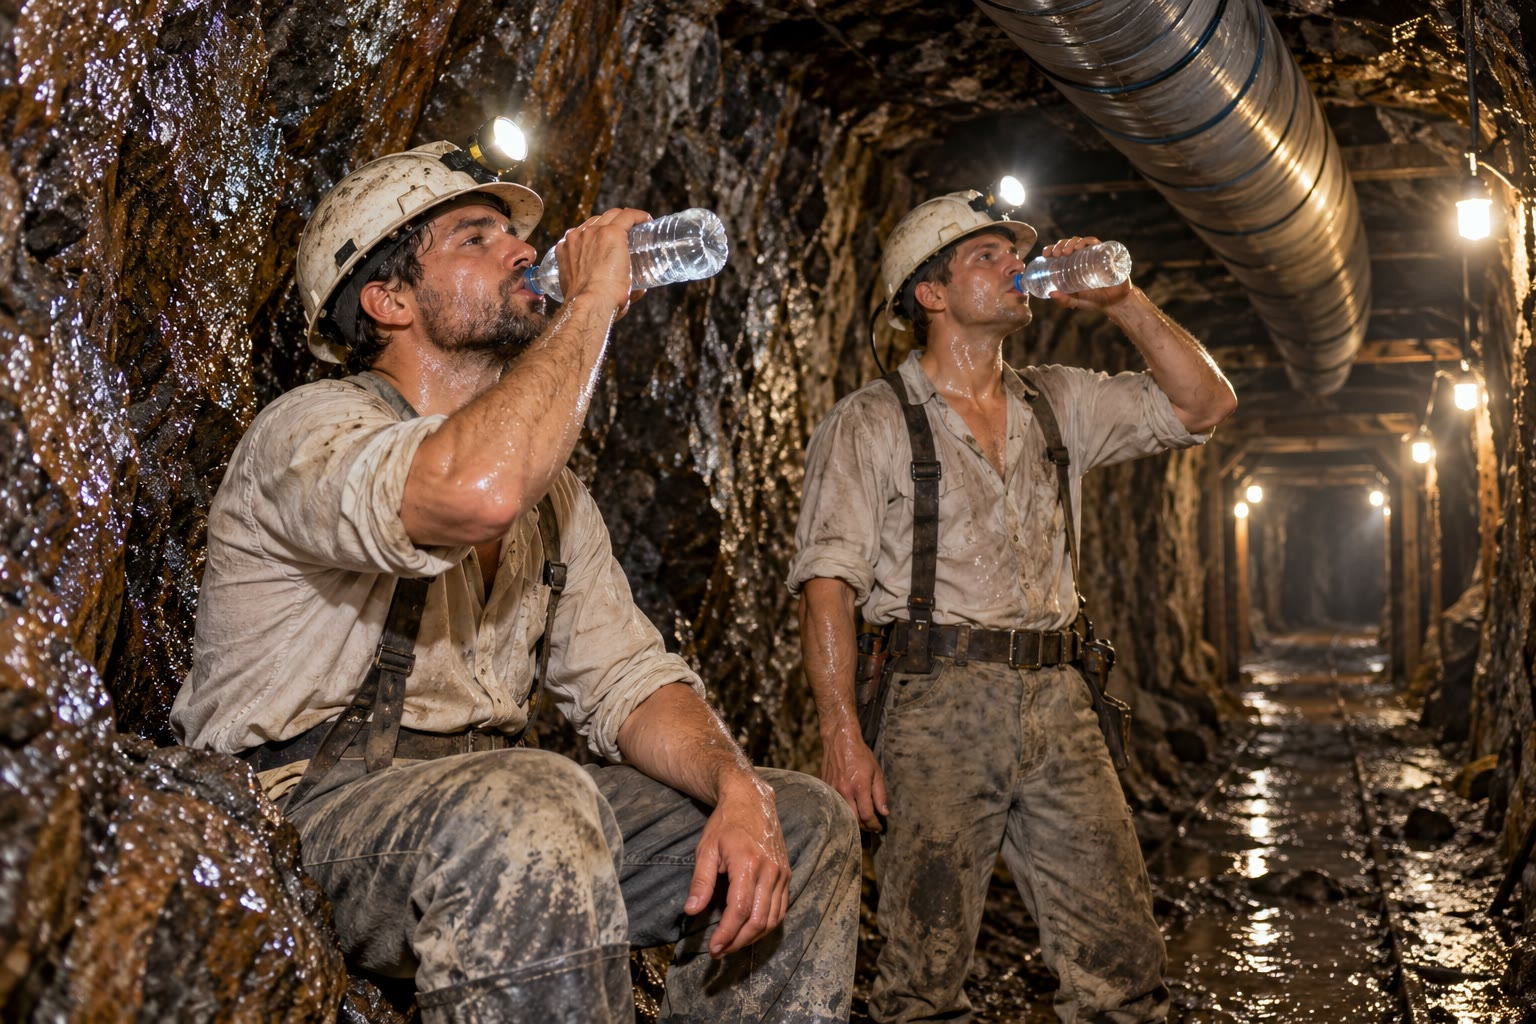
\includegraphics[width=0.62\linewidth]{images/book1/ai/g6-deep-mine.jpg}

{\small عمّال مناجم يشربون في رواق حار، على عمق كيلومترات تحت الأرض.
(رسم بالذكاء الاصطناعي.)}
\end{omfigure}

\begin{recall}
الأرض \omterm{def:g6:earth-a-planet:planet-types}{كوكب صخري}، كرة يبلغ قطرها نحو 12\,742~كيلومترًا: ونصف قطرها، من
السطح إلى المركز، نحو 6371~كيلومترًا
(\cref{ch:g6:earth-a-planet}). وتنتمي صخورها إلى ثلاث عائلات: النارية
والرسوبية والمتحولة (\cref{ch:g6:rocks-and-minerals}). وعند \omterm{def:g4:volcanoes-earthquakes-first-look:volcano}{البركان}، يصعد
\omterm{def:g3:stones-pebbles-sand:rock}{الصخر} المنصهر من الأسفل ويسيل \omterm{def:g4:volcanoes-earthquakes-first-look:eruption}{حممًا}؛ وفي \omterm{def:g4:volcanoes-earthquakes-first-look:earthquake}{الزلزال}، تهتز
الأرض (\cref{ch:g4:volcanoes-earthquakes-first-look}).
\end{recall}
% ledger: earth:Rmean

\section{إلى أي عمق وصلنا؟}

منذ زمن بعيد يحفر الناس في الأرض بحثًا عن الماء والحجارة
والفلزات. ونوعان من الحفر يصلان إلى أبعد عمق.

\textbf{المناجم.} أعمق منجم في العالم منجم ذهب قرب
جوهانسبرغ، في جنوب إفريقيا. وتنزل أروقته إلى أكثر من 4~كيلومترات تحت
السطح. وهناك في الأسفل، تبلغ حرارة الجدران الصخرية نحو 60~درجة مئوية:
ويُبرَّد المنجم بضخ آلاف الأطنان من الجليد الممزوج بالماء إلى الأسفل،
وبمراوح عملاقة تدفع الهواء عبر الأروقة.
% ledger: gwr:deepest-mine

\textbf{ثقوب الحفر.} ثقب الحفر ثقب ضيق تحفره آلة من السطح؛
ولا ينزل فيه أحد. وأعمقها ثقب قصة أول الفصل، الذي حُفر من أجل العلم في
شبه جزيرة كولا، في الشمال الغربي من روسيا:
12\,262~مترًا، أي نحو 12.3~كيلومتر.
% ledger: sciam:kola-depth

تبدو هذه الأعماق هائلة. لكنها، مقارنة بحجم الأرض،
ضئيلة. ويبيّنها الشكل أدناه على شريط واحد، بجانب أعلى
\omterm{def:g1:landscapes-around-us:landform}{جبل}، \omterm{def:g1:landscapes-around-us:landform}{جبل} إفرست (8849~مترًا).
% ledger: tht:everest

\begin{omfigure}
\begin{tikzpicture}[yscale=0.27, xscale=1]
  % sea-level ground and the sky
  \fill[blue!6] (-0.2,0) rectangle (8.6,9.6);
  \fill[brown!35] (-0.2,0) rectangle (8.6,-13.4);
  \draw[thick, brown!60!black] (-0.2,0) -- (8.6,0);
  % depth axis
  \draw[->] (0,-13.4) -- (0,9.9) node[above, font=\scriptsize] {km};
  \foreach \y in {-12,-8,-4,0,4,8} \draw (-0.08,\y) -- (0.08,\y) node[left=2pt, font=\scriptsize] {\y};
  % Everest
  \fill[gray!55] (1.0,0) -- (2.2,8.849) -- (3.4,0) -- cycle;
  \draw[dashed, gray] (0,8.849) -- (2.2,8.849);
  \node[font=\scriptsize, right] at (2.35,8.6) {\foreignlanguage{arabic}{إفرست، ارتفاعه \babelsublr{8.8~km}}};
  % deepest mine
  \draw[line width=2.2pt, black!70] (4.4,0) -- (4.4,-4);
  \draw[dashed, gray] (0,-4) -- (4.4,-4);
  \node[font=\scriptsize, right, align=left] at (4.5,-3.6) {أعمق منجم\\ \foreignlanguage{arabic}{أكثر من \babelsublr{4~km}}};
  % Kola borehole
  \draw[line width=0.7pt, red!75!black] (6.8,0) -- (6.8,-12.262);
  \draw[dashed, gray] (0,-12.262) -- (6.8,-12.262);
  \node[font=\scriptsize, left, align=right, red!60!black] at (6.7,-10.6) {أعمق ثقب حفر\\ \babelsublr{12.3~km}};
  % break and the centre
  \draw[white, line width=3pt] (-0.3,-13.15) -- (8.7,-12.75);
  \draw (-0.3,-13.35) -- (8.7,-12.95);
  \draw (-0.3,-12.95) -- (8.7,-12.55);
  \node[font=\footnotesize, align=center] at (4.2,-16.2) {\foreignlanguage{arabic}{\ldots\ أما مركز الأرض فعلى عمق \babelsublr{6371~km}}\\
     \foreignlanguage{arabic}{وهو على هذا الشريط على بعد نحو 17~مترًا تحت هذا الخط}};
\end{tikzpicture}

{\small الارتفاعات والأعماق مرسومة بمقياس واحد (1~سنتيمتر لكل 3.7~كيلومتر)،
انطلاقًا من \omterm{def:g4:world-physical-map:altitude}{مستوى سطح البحر}. والانقطاع في الشريط يخفي الطريق كله تقريبًا إلى
المركز.}
% ledger: tht:everest, gwr:deepest-mine, sciam:kola-depth, earth:Rmean
\end{omfigure}

\begin{method}[مقارنة عمق بنصف قطر الأرض]\label{met:g6:inside-the-earth:percent}
\begin{enumerate}
  \item اكتب العمق ونصف القطر بالوحدة نفسها (الكيلومتر).
  \item اقسم العمق على نصف القطر، ثم اضرب في 100: فتحصل على
        العمق نسبةً مئوية من الطريق إلى المركز.
  \item لتعرف كم مرة يكون المركز أعمق، اقسم نصف القطر على
        العمق.
\end{enumerate}
\end{method}

\begin{example}[أعمق ثقب حفر]\label{ex:g6:inside-the-earth:kola}
عمق ثقب الحفر 12.3~كيلومتر ونصف القطر 6371~كيلومترًا.
$12.3 \div 6371 \approx 0.0019$، و$0.0019 \times 100 = 0.19$: فقد
قطع الثقب نحو \textbf{0.2~\%} من الطريق إلى المركز. وبالعكس،
$6371 \div 12.3 \approx 518$: فالمركز أعمق من قاع الثقب بأكثر من
500~مرة.

ولأعمق منجم، نحو 4~كيلومترات: $4 \div 6371 \approx 0.0006$، أي
0.06~\%: أقل من ثقب الحفر بثلاث مرات.
% ledger: sciam:kola-depth, earth:Rmean, gwr:deepest-mine
\end{example}

إذن لم يرَ أحد قط باطن الأرض العميق، ولم يلمسه، ولم يأخذ منه عينة.
وما نعرفه عنه يأتي من أدلة أخرى، وأهمها موجات
\omterm{def:g4:volcanoes-earthquakes-first-look:earthquake}{الزلازل} (القسم~\ref{sec:g6:inside-the-earth:waves}).

\section{القشرة والوشاح واللب}

الأرض مبنية طبقات، كما البيضة المسلوقة تقريبًا: قشر رقيق هش،
و«بياض» سميك، و«صفار» في الوسط.
% ledger: usgs:layers-egg

\begin{omfigure}
\begin{tikzpicture}
  % a boiled egg cut in half
  \begin{scope}
    \fill[white] (0,0) ellipse (1.25 and 1.6);
    \draw[brown!50!black, line width=1.6pt] (0,0) ellipse (1.25 and 1.6);
    \fill[yellow!70!orange] (0,-0.15) circle (0.72);
    \node[font=\scriptsize, anchor=west] (s) at (1.8,1.3) {القشر};
    \draw[gray] (s.west) -- (1.0,0.98);
    \node[font=\scriptsize, anchor=west] (w) at (1.8,0.4) {البياض};
    \draw[gray] (w.west) -- (0.95,0.4);
    \node[font=\scriptsize, anchor=west] (y) at (1.8,-0.5) {الصفار};
    \draw[gray] (y.west) -- (0.5,-0.4);
    \node[font=\small] at (0,-2.0) {بيضة مسلوقة};
  \end{scope}
  \draw[->, thick, gray] (3.0,0) -- (4.2,0);
  % the Earth, not to scale
  \begin{scope}[xshift=6.2cm]
    \fill[orange!45!red!45] (0,0) circle (1.55);
    \fill[orange!75!yellow] (0,0) circle (0.95);
    \fill[yellow!55] (0,0) circle (0.42);
    \draw[brown!50!black, line width=1.6pt] (0,0) circle (1.55);
    \node[font=\scriptsize, anchor=west] (c) at (1.95,1.3) {القشرة};
    \draw[gray] (c.west) -- (1.12,1.07);
    \node[font=\scriptsize, anchor=west] (m) at (1.95,0.55) {الوشاح};
    \draw[gray] (m.west) -- (1.2,0.5);
    \node[font=\scriptsize, anchor=west] (o) at (1.95,-0.2) {اللب الخارجي};
    \draw[gray] (o.west) -- (0.7,-0.2);
    \node[font=\scriptsize, anchor=west] (i) at (1.95,-0.9) {اللب الداخلي};
    \draw[gray] (i.west) -- (0.15,-0.25);
    \node[font=\small] at (0,-2.0) {الأرض، بلا مقياس رسم};
  \end{scope}
\end{tikzpicture}

{\small الأرض مقارنةً ببيضة مسلوقة. وخلافًا للصفار، يتكون \omterm{def:g6:inside-the-earth:layers}{اللب} من
جزأين. وفي هذا الرسم تبدو \omterm{def:g6:inside-the-earth:layers}{القشرة} أسمك بكثير مما هي؛ والرسم
بمقياس الرسم يأتي بعده.}
% ledger: usgs:layers-egg
\end{omfigure}

\begin{definition}[طبقات الأرض]\label{def:g6:inside-the-earth:layers}
تتكون الأرض من ثلاث طبقات رئيسية، من السطح إلى المركز:
\begin{itemize}
  \item \emph{القشرة}\index{قشرة}، طبقة خارجية رقيقة من \omterm{def:g3:stones-pebbles-sand:rock}{الصخر} الصلب،
        يتراوح سمكها بين بضعة كيلومترات وبضع عشرات من الكيلومترات؛
  \item \emph{الوشاح}\index{وشاح}، طبقة سميكة من \omterm{def:g3:stones-pebbles-sand:rock}{الصخر} الصلب الحار الكثيف،
        تمتد إلى عمق نحو 2900~كيلومتر؛
  \item \emph{اللب}\index{لب}، وهو من الفلز، معظمه حديد مع شيء من
        النيكل، ويمتد من عمق نحو 2900~كيلومتر إلى المركز. وللب
        جزآن: \emph{اللب الخارجي}\index{لب خارجي}، وهو سائل،
        و\emph{اللب الداخلي}\index{لب داخلي}، وهو كرة صلبة في المركز،
        نصف قطرها نحو 1220~كيلومترًا.
\end{itemize}
% ledger: usgs:layers-egg, usgs:crust-thickness, data:prem, earth:Rmean
\end{definition}

يبيّن الرسم أدناه الطبقات \emph{بمقياس الرسم}، وحدودها كما
قاستها موجات \omterm{def:g4:volcanoes-earthquakes-first-look:earthquake}{الزلازل}.

\begin{omfigure}
\pgfplotstableread{figdata/out/grade-6-earth_layers-disc.dat}\disctab
\pgfplotstablegetelem{0}{r_cm}\of\disctab \let\rE\pgfplotsretval
\pgfplotstablegetelem{1}{r_cm}\of\disctab \let\rOC\pgfplotsretval
\pgfplotstablegetelem{2}{r_cm}\of\disctab \let\rIC\pgfplotsretval
\begin{minipage}[c]{0.43\linewidth}\centering
\begin{tikzpicture}
  \fill[orange!45!red!45] (0,0) circle (\rE cm);
  \fill[orange!75!yellow] (0,0) circle (\rOC cm);
  \fill[yellow!55] (0,0) circle (\rIC cm);
  \draw[brown!50!black, line width=0.45pt] (0,0) circle (\rE cm);
  
  \draw[gray, thin] (-0.25,\rE) rectangle (0.25,\rE-0.12);
  
  \node[font=\scriptsize, align=center, inner sep=0pt] at (0,0) {اللب\\ الداخلي};
  \node[font=\scriptsize, align=center] at (0,1.03) {اللب\\ الخارجي};
  \node[font=\scriptsize] at (0,2.12) {الوشاح};
  \draw[<-, font=\scriptsize] (1.98,1.98) -- (2.3,2.75) node[above, align=center] {القشرة\\ \foreignlanguage{arabic}{(خط رفيع)}};
\end{tikzpicture}
\end{minipage}\hfill
\begin{minipage}[c]{0.55\linewidth}\centering
\begin{tikzpicture}[yscale=0.034, xscale=0.55]
  % the top 100 km enlarged: ocean on the left, continent and a range on the right
  \fill[orange!45!red!45] (0,0) rectangle (12,-100);
  \fill[blue!25] (0,0) rectangle (4,-4);
  \fill[brown!45] (0,-4) rectangle (4,-9);                 % oceanic crust 5 km
  \fill[brown!60] (4,0) -- (4,-9) -- (5,-30) -- (8,-30) -- (9,-100) -- (11,-100) -- (11.4,-30) -- (12,-30) -- (12,0) -- cycle;
  \fill[brown!60] (8.6,0) -- (10,5) -- (11.4,0) -- cycle;   % the range (not to scale above ground)
  \draw[red!75!black, line width=0.8pt] (6.2,0) -- (6.2,-12.262);
  \draw[thin] (0,0) rectangle (12,-100);
  \foreach \y in {0,-20,-40,-60,-80,-100} \draw (0,\y) -- (-0.2,\y) node[left, font=\scriptsize] {\pgfmathparse{-\y}\pgfmathprintnumber{\pgfmathresult}};
  \node[font=\scriptsize, rotate=90] at (-2.0,-50) {\foreignlanguage{arabic}{العمق \babelsublr{(km)}}};
  \node[font=\scriptsize, align=center] at (2,-44) {قشرة\\ محيطية\\ \babelsublr{5~km}};
  \draw[->, thin] (2,-29) -- (2,-8);
  \node[font=\scriptsize, align=center] at (6.6,-21) {قشرة قارية\\ \babelsublr{30~km}};
  \node[font=\scriptsize, align=center] at (10.0,-50) {جذر\\ سلسلة جبلية\\ \foreignlanguage{arabic}{حتى}\\ \babelsublr{100~km}};
  \node[font=\scriptsize, align=center, red!60!black] at (7.4,-6.5) {ثقب الحفر};
  \node[font=\scriptsize] at (4.5,-75) {الوشاح};
  \node[font=\scriptsize, blue!60!black] at (2,2.5) {المحيط};
\end{tikzpicture}
\end{minipage}

\smallskip
{\small إلى اليمين: الأرض مقطوعة، بمقياس الرسم؛ والمربع الرمادي الصغير في الأعلى
يحدد الجزء المكبَّر إلى اليسار. إلى اليسار: أعلى 100~كيلومتر، مكبَّرة نحو
60~مرة: \omterm{def:g6:inside-the-earth:layers}{قشرة} رقيقة تحت المحيطات، \omterm{def:g6:inside-the-earth:layers}{وقشرة} أسمك تحت \omterm{def:g3:continents-and-oceans:continent}{القارات}،
وأسمك ما تكون تحت \omterm{def:g4:world-physical-map:range}{السلاسل الجبلية} العالية؛ وثقب الحفر القياسي بالأحمر.}
% ledger: data:prem, earth:Rmean, usgs:crust-thickness, sciam:kola-depth (figdata/grade-6/earth_layers.py)
\end{omfigure}

\begin{center}\small
\begin{tabular}{|l|c|c|c|l|}
\hline
\textbf{الطبقة} & \textbf{من (km)} & \textbf{إلى (km)} & \textbf{السمك (km)} & \textbf{مكوَّنة من} \\
\hline
\omterm{def:g6:inside-the-earth:layers}{القشرة} & 0 & من 5 إلى 100 & من 5 إلى 100 & \omterm{def:g3:stones-pebbles-sand:rock}{صخر} صلب \\
\omterm{def:g6:inside-the-earth:layers}{الوشاح} & قاعدة \omterm{def:g6:inside-the-earth:layers}{القشرة} & 2891 & نحو 2860 & \omterm{def:g3:stones-pebbles-sand:rock}{صخر} صلب، حار جدًا \\
\omterm{def:g6:inside-the-earth:layers}{اللب الخارجي} & 2891 & 5150 & نحو 2260 & فلز سائل \\
\omterm{def:g6:inside-the-earth:layers}{اللب الداخلي} & 5150 & 6371 (المركز) & نحو 1220 & فلز صلب \\
\hline
\end{tabular}
\end{center}
% ledger: data:prem, usgs:crust-thickness, usgs:layers-egg, earth:Rmean (figdata/grade-6/earth_layers.py, main table)

\textbf{\omterm{def:g6:inside-the-earth:layers}{القشرة}} هي الطبقة الوحيدة التي نستطيع أن نمشي عليها ونحفر فيها. وهي
رقيقة جدًا مقارنة بالطبقات الأخرى: فتحت المحيطات لا يتجاوز سمكها نحو 5~كيلومترات؛
وتحت \omterm{def:g3:continents-and-oceans:continent}{القارات}، نحو 30~كيلومترًا في المتوسط؛ وتحت \omterm{def:g4:world-physical-map:range}{السلاسل الجبلية} العالية
مثل \omterm{def:g1:landscapes-around-us:landform}{جبال} الألب، قد تنزل قاعدتها إلى عمق 100~كيلومتر، كجذر
السن. وحتى ثقب الحفر القياسي، بعمقه البالغ 12.3~كيلومتر، لم يقطع نصف \omterm{def:g6:inside-the-earth:layers}{قشرة} قارية متوسطة. وفي الرسم بمقياس الرسم، تكون \omterm{def:g6:inside-the-earth:layers}{القشرة}
أرق من الخط \omterm{def:g2:water-on-earth:ocean}{المحيط} بالقرص.
% ledger: usgs:crust-thickness, sciam:kola-depth

\textbf{\omterm{def:g6:inside-the-earth:layers}{الوشاح}} أسمك الطبقات: يمتد من قاعدة
\omterm{def:g6:inside-the-earth:layers}{القشرة} إلى عمق 2891~كيلومترًا، أي نحو 45~\% من الطريق إلى المركز. وصخره
صلب، لكنه حار جدًا وأكثف من \omterm{def:g3:stones-pebbles-sand:rock}{صخر} \omterm{def:g6:inside-the-earth:layers}{القشرة}. وعلى مدى ملايين
السنين، يمكن \omterm{def:g3:stones-pebbles-sand:rock}{للصخر} الحار في جزء من \omterm{def:g6:inside-the-earth:layers}{الوشاح} أن يزحف ببطء شديد، كعجينة
شديدة القساوة.
% ledger: data:prem, usgs:layers-egg, usgs:lithosphere-80km

\textbf{\omterm{def:g6:inside-the-earth:layers}{اللب}} يبدأ عند عمق 2891~كيلومترًا ويمتد إلى المركز. وهو
ليس من \omterm{def:g3:stones-pebbles-sand:rock}{الصخر} بل من الفلز: سبيكة من الحديد والنيكل، كثافتها تقارب ضعف
كثافة \omterm{def:g6:inside-the-earth:layers}{الوشاح}. وجزؤه الخارجي \emph{سائل}: \omterm{def:g2:water-on-earth:ocean}{محيط} من الفلز المنصهر
عمقه أكثر من 2000~كيلومتر. أما جزؤه الداخلي، من عمق 5150~كيلومترًا إلى
المركز، فكرة \emph{صلبة} من الفلز، نصف قطرها نحو 1220~كيلومترًا: أي نحو 70~\% من عرض القمر. وحين تدور الأرض، يتحرك الفلز السائل في
\omterm{def:g6:inside-the-earth:layers}{اللب الخارجي}، وهذه الحركة تصنع المجال المغناطيسي للأرض، ذلك
الذي يدير إبرة البوصلة.
% ledger: data:prem, usgs:layers-egg, earth:Rmean, planet:Moon.diameter

كلما ازداد العمق ازدادت الكثافة. فكثافة الماء 1~غرام لكل سنتيمتر
مكعب: \omterm{def:g3:stones-pebbles-sand:rock}{وصخر} \omterm{def:g6:inside-the-earth:layers}{القشرة} أكثف منه بما بين 2.6 و2.9 مرة،
\omterm{def:g3:stones-pebbles-sand:rock}{وصخر} قاع \omterm{def:g6:inside-the-earth:layers}{الوشاح} بأكثر من 5~مرات، والفلز في
المركز بنحو 13~مرة (انظر المنحنى أدناه). فأثقل المواد في المركز وأخفها في الأعلى: الأرض مرتبة، من \omterm{def:g6:inside-the-earth:layers}{القشرة} الخفيفة إلى \omterm{def:g6:inside-the-earth:layers}{اللب} الفلزي الثقيل.
% ledger: data:prem


\begin{omfigure}
\begin{tikzpicture}
  \begin{axis}[omrecord, width=0.86\linewidth, height=5.4cm,
      xmin=0, xmax=6371, ymin=0, ymax=14,
      xlabel={\foreignlanguage{arabic}{العمق تحت السطح \babelsublr{(km)}}},
      ylabel={\foreignlanguage{arabic}{الكثافة \babelsublr{(g/cm$^3$)}}},
      xtick={0,1000,2000,3000,4000,5000,6000},
      scaled x ticks=false, x tick label style={/pgf/number format/1000 sep={}},
      clip=false]
    \fill[orange!45!red!20] (axis cs:24.4,0) rectangle (axis cs:2891,14);
    \fill[orange!75!yellow!35] (axis cs:2891,0) rectangle (axis cs:5149.5,14);
    \fill[yellow!30] (axis cs:5149.5,0) rectangle (axis cs:6371,14);
    \addplot[very thick, black] table[x=depth_km, y=rho] {figdata/out/grade-6-earth_layers-profile.dat};
    \node[font=\scriptsize] at (axis cs:1450,12.5) {الوشاح};
    \node[font=\scriptsize] at (axis cs:4020,4.5) {اللب الخارجي};
    \node[font=\scriptsize] at (axis cs:5760,4.5) {اللب الداخلي};
    \node[font=\scriptsize, align=left, anchor=west] at (axis cs:80,1.4) {\foreignlanguage{arabic}{القشرة: من \babelsublr{2.6} إلى \babelsublr{2.9}}};
  \end{axis}
\end{tikzpicture}

{\small كثافة الأرض عند كل عمق، بحسب نموذج مرجعي بُني
من قياسات \omterm{def:g4:volcanoes-earthquakes-first-look:earthquake}{الزلازل}. وتقفز الكثافة من نحو 5.6 إلى نحو
9.9~غرام لكل \babelsublr{cm$^3$} حيث يُخلي \omterm{def:g3:stones-pebbles-sand:rock}{صخر} \omterm{def:g6:inside-the-earth:layers}{الوشاح} المكان لفلز
\omterm{def:g6:inside-the-earth:layers}{اللب}.}
% ledger: data:prem (figdata/grade-6/earth_layers.py, part profile)
\end{omfigure}

\begin{inthelab}[طبقات في كأس (في القسم، مع المعلم)]
يصب المعلم، ببطء وواحدًا بعد الآخر، في كأس طويلة:
قليلًا من العسل، وقليلًا من الماء الملوّن بقطرة حبر، وقليلًا من زيت الطبخ.
وأيًّا كان ترتيب الصب، يستقر العسل بعد لحظة في
القاع، والماء في الوسط، والزيت في الأعلى: فكل سائل يستقر
تحت السوائل الأخف منه وفوق السوائل الأكثف منه. وإذا رُجّت الكأس تعكّرت؛
وإذا تُركت وشأنها، ترتبت من جديد. والأرض مرتبة طبقات بالطريقة نفسها: فأكثف المواد، فلز \omterm{def:g6:inside-the-earth:layers}{اللب}، في المركز، وأخف \omterm{def:g3:stones-pebbles-sand:rock}{الصخور} في الأعلى.
\end{inthelab}


\begin{remark}[ما مدى رقة القشرة؟]\label{rem:g6:inside-the-earth:thin-crust}
على \omterm{def:g3:continents-and-oceans:globe}{مجسم} مدرسي للكرة الأرضية قطره 30~سنتيمترًا، يكون سمك \omterm{def:g6:inside-the-earth:layers}{القشرة} القارية (30~كيلومترًا)
نحو 0.7~مليمتر، \omterm{def:g6:inside-the-earth:layers}{والقشرة} المحيطية (5~كيلومترات) بسمك
ورقة تقريبًا. \omterm{def:g6:inside-the-earth:layers}{فالقشرة} أقل من نصف واحد في
المئة من نصف القطر: $30 \div 6371 \approx 0.0047$، أي 0.47~\%.
% ledger: usgs:crust-thickness, earth:Rmean
\end{remark}

\section{كيف تخبرنا موجات الزلازل بالباقي}\label{sec:g6:inside-the-earth:waves}

إذا لم ينزل أحد أعمق من 12~كيلومترًا، فكيف نستطيع أن نرسم \omterm{def:g6:inside-the-earth:layers}{اللب}؟ الجواب
يأتي من \omterm{def:g4:volcanoes-earthquakes-first-look:earthquake}{الزلازل}. فحين يهز \omterm{def:g4:volcanoes-earthquakes-first-look:earthquake}{زلزال} الأرض، تنطلق منه موجات
في كل الاتجاهات وتنتقل \emph{عبر} الأرض كلها، كما ينتقل
صوت طرقة عبر جدار. وتسجّل أجهزة في أماكن كثيرة حول العالم وقت وصول كل موجة (ستتعرف عليها في
\cref{ch:g7:earthquakes}).
% ledger: data:prem

لا تنتقل الموجات بالسرعة نفسها في كل المواد. فحين
تصل إلى الحد الفاصل بين طبقتين، تتغير سرعتها فجأة: فبعض
الموجات يرتد، وبعضها ينحرف وهو يعبر، كما يحدث للضوء حين يدخل
الماء. وبتوقيت موجات \omterm{def:g4:volcanoes-earthquakes-first-look:earthquake}{زلازل} كثيرة، في محطات حول الكرة الأرضية كلها، وجد العلماء أين تقع هذه الحدود،
وأي الطبقات صلبة وأيها سائلة. ويسمي علماء \omterm{def:g4:volcanoes-earthquakes-first-look:earthquake}{الزلازل} النوعين الرئيسيين من
الموجات \emph{الموجات P} (الأسرع، وهي تدفع \omterm{def:g3:stones-pebbles-sand:rock}{الصخر} وتشده)
و\emph{الموجات S} (الأبطأ، وهي تهزه من جانب إلى جانب)؛ وستدرسها
مجلدات لاحقة عن قرب. وللموجات S خاصية لافتة: فهي
لا تستطيع أن تنتقل عبر السائل.

\begin{omfigure}
\begin{tikzpicture}
  \begin{axis}[omrecord, width=0.86\linewidth, height=5.4cm,
      xmin=0, xmax=6371, ymin=0, ymax=14.5,
      xlabel={\foreignlanguage{arabic}{العمق تحت السطح \babelsublr{(km)}}},
      ylabel={\foreignlanguage{arabic}{سرعة الموجة \babelsublr{(km/s)}}},
      xtick={0,1000,2000,3000,4000,5000,6000},
      scaled x ticks=false, x tick label style={/pgf/number format/1000 sep={}},
      clip=false]
    \fill[orange!45!red!20] (axis cs:24.4,0) rectangle (axis cs:2891,14.5);
    \fill[orange!75!yellow!35] (axis cs:2891,0) rectangle (axis cs:5149.5,14.5);
    \fill[yellow!30] (axis cs:5149.5,0) rectangle (axis cs:6371,14.5);
    \addplot[very thick, blue!70!black] table[x=depth_km, y=vp] {figdata/out/grade-6-earth_layers-profile.dat};
    \addplot[very thick, red!75!black] table[x=depth_km, y=vs] {figdata/out/grade-6-earth_layers-profile.dat};
    \node[font=\scriptsize, blue!70!black, anchor=south] at (axis cs:1300,12.9) {\foreignlanguage{arabic}{الموجات P، وهي الأسرع}};
    \node[font=\scriptsize, red!75!black, anchor=north] at (axis cs:1500,6.1) {\foreignlanguage{arabic}{الموجات S، وهي الأبطأ}};
    \node[font=\scriptsize, red!75!black, align=center, fill=white, fill opacity=0.8, text opacity=1] at (axis cs:4020,1.9) {\foreignlanguage{arabic}{الموجات S: صفر}\\ \foreignlanguage{arabic}{(سائل)}};
    \node[font=\scriptsize] at (axis cs:4020,13.6) {اللب الخارجي};
    \node[font=\scriptsize] at (axis cs:5760,13.6) {اللب الداخلي};
    \node[font=\scriptsize] at (axis cs:1450,1.5) {الوشاح};
  \end{axis}
\end{tikzpicture}

{\small سرعة نوعي موجات \omterm{def:g4:volcanoes-earthquakes-first-look:earthquake}{الزلازل} عند كل عمق، في
النموذج المرجعي نفسه. وفي \omterm{def:g6:inside-the-earth:layers}{اللب الخارجي} تتوقف الموجات S: فسرعتها
صفر، لأن \omterm{def:g6:inside-the-earth:layers}{اللب الخارجي} سائل.}
% ledger: data:prem (figdata/grade-6/earth_layers.py, part profile)
\end{omfigure}

لنقرأ المنحنى من اليسار إلى اليمين: في \omterm{def:g6:inside-the-earth:layers}{الوشاح}، يزداد نوعا الموجات
سرعة كلما ازداد العمق. وعند عمق 2891~كيلومترًا، تختفي الموجات S
وتتباطأ الموجات P فجأة: هذه قمة \omterm{def:g6:inside-the-earth:layers}{اللب الخارجي} السائل. وعند عمق
5150~كيلومترًا، تعود الموجات P إلى التسارع وتظهر الموجات S من جديد: هذا
هو \omterm{def:g6:inside-the-earth:layers}{اللب الداخلي} الصلب.
% ledger: data:prem

\begin{history}[إنغه ليمان واللب الداخلي]
\begin{minipage}[c]{0.72\linewidth}
في أوائل ثلاثينيات القرن العشرين، كان علماء \omterm{def:g4:volcanoes-earthquakes-first-look:earthquake}{الزلازل} يظنون أن للأرض طبقتين: وشاحًا صلبًا حول \omterm{def:g6:inside-the-earth:layers}{لب} سائل. ودرست عالمة \omterm{def:g4:volcanoes-earthquakes-first-look:earthquake}{الزلازل} الدنماركية إنغه ليمان موجات
\omterm{def:g4:volcanoes-earthquakes-first-look:earthquake}{زلزال} قوي ضرب نيوزيلندا عام 1929، سجّلتها محطات
بعيدة. فبعض الموجات وصل إلى أماكن ما كان ينبغي أن يصل إليها أبدًا لو كان
\omterm{def:g6:inside-the-earth:layers}{اللب} سائلًا كله. وفي مقال نشرته عام 1936، عنوانه ببساطة «P\,$'$»،
اقترحت تفسيرًا: داخل \omterm{def:g6:inside-the-earth:layers}{اللب} السائل يوجد
\emph{\omterm{def:g6:inside-the-earth:layers}{لب داخلي} صلب} أصغر، يرد هذه الموجات. وكتبت بتواضع
أن المعطيات «غير كافية تمامًا» للتأكد، لكن
التفسير «يبدو ممكنًا»، وطلبت من باحثين آخرين أن يختبروه.
وقد فعلوا، واليوم صار \omterm{def:g6:inside-the-earth:layers}{اللب الداخلي} الصلب جزءًا من كل نموذج مرجعي للأرض، مثل النموذج المستعمل في منحنيات هذا الفصل.
% ledger: nbi:lehmann-1936
\end{minipage}\hfill
\begin{minipage}[c]{0.24\linewidth}\centering
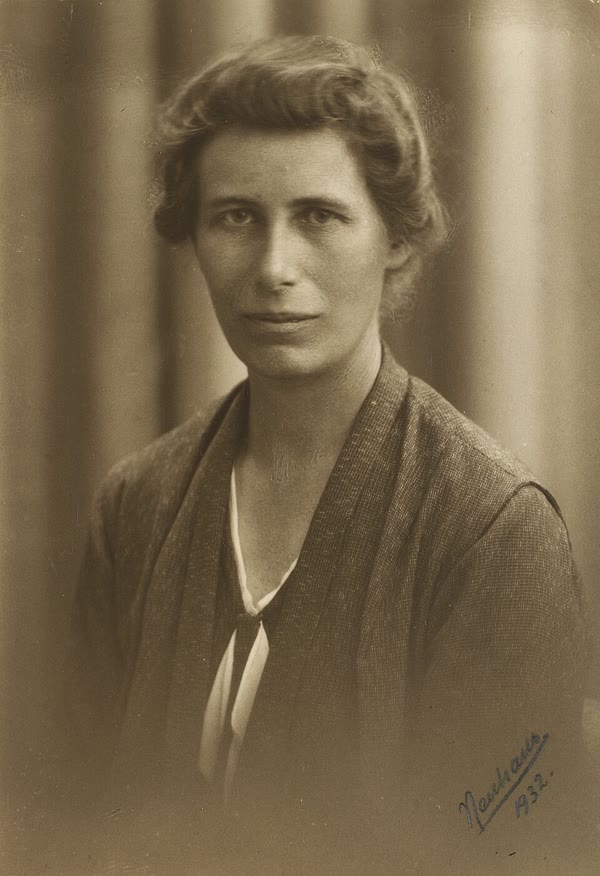
\includegraphics[width=\linewidth]{images/book1/g6-inge-lehmann.jpg}\\[2pt]
{\footnotesize إنغه ليمان عام 1932. (الصورة: إيفن نويهاوس، ملك عام،
عبر ويكيميديا كومنز.)}
% ledger: commons:inge-lehmann
\end{minipage}
\end{history}

\section{كلما ازداد العمق ازدادت الحرارة}

كل منجم عميق وكل ثقب حفر عميق يُظهر الشيء نفسه: كلما نزلنا
أعمق، ازدادت حرارة \omterm{def:g3:stones-pebbles-sand:rock}{الصخر}. ففي أعمق منجم، تبلغ حرارة الجدران الصخرية
نحو 60~درجة مئوية، على عمق يزيد على 4~كيلومترات؛ وفي قاع ثقب الحفر
القياسي، على عمق 12.3~كيلومتر، كانت حرارة \omterm{def:g3:stones-pebbles-sand:rock}{الصخر} نحو 180~درجة.
% ledger: gwr:deepest-mine, sciam:kola-180C

قرب السطح، ترتفع درجة الحرارة بمعدل منتظم إلى حد ما. ففي
الولايات المتحدة، جمع العلماء قياسات 284 ثقب حفر،
معظمها أعمق من 600~متر. وفي المتوسط، ارتفعت درجة الحرارة
\textbf{29~درجة لكل كيلومتر} من العمق: نحو 25~درجة لكل
كيلومتر في شرق البلاد و34 في غربها. لكن المعدل
يختلف كثيرًا من مكان إلى آخر: ففي تلك الثقوب، تراوح بين 6
و69~درجة لكل كيلومتر.
% ledger: usgs:gradient-29

\begin{omfigure}
\begin{tikzpicture}
  \begin{axis}[omrecord, omdepth, width=0.78\linewidth, height=5.6cm,
      xmin=0, xmax=160, ymin=0, ymax=2,
      xlabel={\foreignlanguage{arabic}{درجة حرارة الصخر \babelsublr{($^\circ$C)}}},
      ylabel={\foreignlanguage{arabic}{العمق \babelsublr{(km)}}},
      ytick={0,0.5,1,1.5,2},
      yticklabel style={/pgf/number format/fixed},
      legend pos=north east, legend cell align=left,
            legend style={font=\scriptsize},
      clip=false]
    \addplot[forget plot, name path=lo, thin, gray] table[x=t_low, y=depth_km] {figdata/out/grade-6-earth_layers-geotherm.dat};
    \addplot[forget plot, name path=hi, thin, gray] table[x=t_high, y=depth_km] {figdata/out/grade-6-earth_layers-geotherm.dat};
    \addplot[forget plot, gray!20] fill between[of=lo and hi];
    \addplot[forget plot, thick, blue!70!black] table[x=t_east, y=depth_km] {figdata/out/grade-6-earth_layers-geotherm.dat};
    \addplot[forget plot, very thick, black] table[x=t_mean, y=depth_km] {figdata/out/grade-6-earth_layers-geotherm.dat};
    \addplot[forget plot, thick, red!75!black] table[x=t_west, y=depth_km] {figdata/out/grade-6-earth_layers-geotherm.dat};
    \addlegendimage{area legend, fill=gray!20, draw=gray}
    \addlegendentry{\foreignlanguage{arabic}{كل الثقوب: من 6 إلى \babelsublr{69~$^\circ$C} لكل كيلومتر}}
    \addlegendimage{thick, blue!70!black}\addlegendentry{\foreignlanguage{arabic}{الشرق: \babelsublr{25~$^\circ$C} لكل كيلومتر}}
    \addlegendimage{very thick, black}\addlegendentry{\foreignlanguage{arabic}{المتوسط: \babelsublr{29~$^\circ$C} لكل كيلومتر}}
    \addlegendimage{thick, red!75!black}\addlegendentry{\foreignlanguage{arabic}{الغرب: \babelsublr{34~$^\circ$C} لكل كيلومتر}}
  \end{axis}
\end{tikzpicture}

{\small درجة الحرارة بحسب العمق (نحو الأسفل) لأرض تبدأ حرارتها عند
\babelsublr{15~$^\circ$C}، بالمعدل المتوسط (29، بالأسود)، ومتوسطي الشرق والغرب
(25 و34) والمدى المقيس كله (من 6 إلى 69، الشريط الرمادي). وتصل
القياسات إلى نحو 2~كيلومتر.}
% ledger: usgs:gradient-29, planet:Earth.Tmean (figdata/grade-6/earth_layers.py, part geotherm)
\end{omfigure}

\begin{method}[درجة الحرارة على عمق معيّن]\label{met:g6:inside-the-earth:temperature}
\begin{enumerate}
  \item خذ درجة حرارة الأرض قرب السطح.
  \item اضرب العمق، بالكيلومترات، في المعدل، بالدرجات لكل
        كيلومتر: فتعرف بكم تزداد الحرارة.
  \item اجمع العددين. ولا تستعمل ذلك إلا في المدى الذي قيس فيه المعدل:
        بضعة كيلومترات.
\end{enumerate}
\end{method}

\begin{example}[على عمق كيلومترين]\label{ex:g6:inside-the-earth:two-km}
الأرض عند \babelsublr{15~$^\circ$C} والمعدل 29~درجة لكل كيلومتر.
على عمق 2~كيلومتر: $2 \times 29 = 58$ درجة زيادة، إذن $15 + 58 = 73~^\circ$C:
أحر من أحر حمّام، وأحر بكثير من أن تُلمس.
% ledger: usgs:gradient-29, planet:Earth.Tmean
\end{example}

هل يمكن استعمال المعدل نفسه حتى المركز؟ لا. فبمعدل 29~درجة لكل
كيلومتر، ستكون حرارة المركز نحو 185\,000~درجة، وهذا
مستحيل: فالمعدل المقيس في الكيلومترات الأولى لا يصح في الأعماق، حيث يجب أن يكون الارتفاع أبطأ بكثير. ويقدّر العلماء درجة حرارة
\omterm{def:g6:inside-the-earth:layers}{اللب} بطريقة أخرى: ففي المختبر، يضغطون حبيبات دقيقة من
الحديد بين ماستين، حتى يبلغ الضغط ملايين أضعاف ضغط الهواء،
ويسخنونها بأشعة الليزر حتى تنصهر. وبهذه الطريقة، وجدوا أن
درجة الحرارة عند حافة \omterm{def:g6:inside-the-earth:layers}{اللب الداخلي} الصلب نحو
\textbf{6000~درجة مئوية}، ومع ذلك يبقى حديد \omterm{def:g6:inside-the-earth:layers}{اللب الداخلي} صلبًا، لأن الضغط هناك، وهو نحو
3.3~مليون ضعف ضغط الهواء، يمنعه من الانصهار.
% ledger: esrf:core-6000C, usgs:gradient-29

\begin{remark}[حار، ومع ذلك صلب]\label{rem:g6:inside-the-earth:pressure}
إذا ضُغطت مادة بقوة، لم تنصهر إلا عند درجة حرارة أعلى. \omterm{def:g6:inside-the-earth:layers}{فالوشاح}
حار جدًا، ومع ذلك يبقى صلبًا؛ \omterm{def:g6:inside-the-earth:layers}{واللب الخارجي} سائل؛ \omterm{def:g6:inside-the-earth:layers}{واللب الداخلي}،
وهو أحر منهما، صلب من جديد، لأنه أشد الطبقات انضغاطًا.
فانصهار المادة أو عدمه يتوقف على درجة الحرارة \emph{وعلى} الضغط.
% ledger: esrf:core-6000C, data:prem
\end{remark}

\section{تمارين}

\begin{exercise}[$\star$]\label{exo:g6:inside-the-earth:1}
سمِّ طبقات الأرض الأربع بالترتيب، من السطح إلى
المركز. أيها سائلة؟ وأيها مكوَّنة من الفلز؟
\end{exercise}

\begin{exercise}[$\star$]\label{exo:g6:inside-the-earth:2}
صواب أم خطأ؟ صحّح الجمل الخاطئة.
(أ) \omterm{def:g6:inside-the-earth:layers}{القشرة} أسمك تحت المحيطات منها تحت \omterm{def:g3:continents-and-oceans:continent}{القارات}.
(ب) \omterm{def:g6:inside-the-earth:layers}{اللب} مكوَّن من \omterm{def:g3:stones-pebbles-sand:rock}{الصخر}.
(ج) \omterm{def:g6:inside-the-earth:layers}{اللب الداخلي} صلب.
(د) عمق أعمق ثقب حفر حُفر على الإطلاق نحو 12~كيلومترًا.
\end{exercise}

\begin{exercise}[$\star$]\label{exo:g6:inside-the-earth:3}
استعمل جدول الطبقات. (أ) على أي عمق يبدأ \omterm{def:g6:inside-the-earth:layers}{اللب}؟
(ب) على أي عمق يبدأ \omterm{def:g6:inside-the-earth:layers}{اللب الداخلي}؟ (ج) ما سمك \omterm{def:g6:inside-the-earth:layers}{اللب
الخارجي}؟
\end{exercise}

\begin{exercise}[$\star$]\label{exo:g6:inside-the-earth:4}
كثيرًا ما تُقارن الأرض ببيضة مسلوقة. انقل وأكمل: «القشر
يشبه \ldots، والبياض يشبه \ldots{} والصفار يشبه
\ldots{}. لكن خلافًا للصفار، يتكون \ldots{} من جزأين: \ldots{}
سائل و\ldots{} صلب.»
\end{exercise}

\begin{exercise}[$\star\star$]\label{exo:g6:inside-the-earth:5}
\omterm{def:g4:world-physical-map:altitude}{ارتفاع} \omterm{def:g1:landscapes-around-us:landform}{جبل} إفرست 8.849~كيلومتر ونصف قطر الأرض 6371~كيلومترًا. كم
يبلغ \omterm{def:g4:world-physical-map:altitude}{ارتفاع} إفرست نسبةً مئوية من نصف القطر؟ قرّب إلى منزلتين عشريتين.
هل سطح الأرض شديد التضرس إذا نظرنا إليه من بعيد؟
\end{exercise}

\begin{exercise}[$\star\star$]\label{exo:g6:inside-the-earth:6}
سمك \omterm{def:g6:inside-the-earth:layers}{القشرة} القارية 30~كيلومترًا في المتوسط وسمك \omterm{def:g6:inside-the-earth:layers}{القشرة} المحيطية
5~كيلومترات. (أ) كم مرة تكون \omterm{def:g6:inside-the-earth:layers}{القشرة} القارية أسمك؟ (ب) تحت \omterm{def:g4:world-physical-map:range}{سلسلة جبلية}
عالية، قد يبلغ سمك \omterm{def:g6:inside-the-earth:layers}{القشرة} 100~كيلومتر. فكم مرة يكون ذلك أسمك من
\omterm{def:g6:inside-the-earth:layers}{القشرة} المحيطية؟
\end{exercise}

\begin{exercise}[$\star\star$]\label{exo:g6:inside-the-earth:7}
في منطقة ما، حرارة الأرض \babelsublr{12~$^\circ$C} وترتفع درجة الحرارة بمقدار
25~درجة لكل كيلومتر. ما درجة الحرارة (أ) على عمق 1~كيلومتر، (ب) على عمق
1.5~كيلومتر، (ج) على عمق 2~كيلومتر؟
\end{exercise}

\begin{exercise}[$\star\star$]\label{exo:g6:inside-the-earth:8}
في ثقب حفر، حرارة \omterm{def:g3:stones-pebbles-sand:rock}{الصخر} \babelsublr{14~$^\circ$C} قرب السطح
و\babelsublr{74~$^\circ$C} على عمق 2~كيلومتر. بكم درجة ترتفع درجة الحرارة
لكل كيلومتر؟ هل يقع هذا المعدل بين متوسطي الشرق
والغرب في قياسات الفصل؟
\end{exercise}

\begin{exercise}[$\star\star$]\label{exo:g6:inside-the-earth:9}
استعمل منحنى سرعات الموجات. (أ) ما سرعة الموجات P فوق
\omterm{def:g6:inside-the-earth:layers}{اللب} مباشرة، على عمق نحو 2890~كيلومترًا، وتحت قمة \omterm{def:g6:inside-the-earth:layers}{اللب} مباشرة؟
(ب) بين أي عمقين تكون سرعة الموجات S صفرًا؟ (ج) ماذا
يخبرنا ذلك عن هذه الطبقة؟
\end{exercise}

\begin{exercise}[$\star\star$]\label{exo:g6:inside-the-earth:10}
عمق ثقب الحفر القياسي 12.3~كيلومتر. (أ) ما النسبة المئوية التي قطعها من \omterm{def:g6:inside-the-earth:layers}{قشرة}
قارية متوسطة (30~كيلومترًا)؟ (ب) هل وصل إلى \omterm{def:g6:inside-the-earth:layers}{الوشاح}؟
\end{exercise}

\begin{exercise}[$\star\star\star$]\label{exo:g6:inside-the-earth:11}
يقول ليو: «قرب السطح، ترتفع درجة الحرارة بمقدار 29~درجة لكل
كيلومتر، إذن في المركز، على عمق 6371~كيلومترًا، يجب أن تكون
$15 + 29 \times 6371$ درجة.» (أ) احسب عدد ليو. (ب) قارنه
بدرجة الحرارة التي وُجدت في المختبر لحافة \omterm{def:g6:inside-the-earth:layers}{اللب
الداخلي}. (ج) ما الخطأ في استدلال ليو؟
\end{exercise}

\begin{exercise}[$\star\star\star$]\label{exo:g6:inside-the-earth:12}
متوسط كثافة الأرض كلها نحو 5.5~غرام لكل سنتيمتر
مكعب (\cref{ch:g6:earth-a-planet})، لكن كثافة \omterm{def:g3:stones-pebbles-sand:rock}{صخور} \omterm{def:g6:inside-the-earth:layers}{القشرة}
لا تتجاوز ما بين 2.6 و2.9. (أ) ماذا يخبرنا ذلك عن المادة الموجودة
في الأعماق؟ (ب) استعمل منحنى الكثافة: في أي الطبقات تكون الكثافة أكبر من 5.5 في كل مكان؟ (ج) لماذا من المنطقي أن يكون الفلز الثقيل في
المركز لا على السطح؟
\end{exercise}

\section{مسألة: رحلة إلى المركز، بمقياس الرسم}

\begin{problem}[{مسألة نهاية الأسبوع --- نموذج للأرض قطره 2~متر:
الطبقات، وأعمق الحفر، والباطن الحار، مرسومة بمقياس الرسم}]
\label{pb:g6:inside-the-earth:1}
% ledger: earth:Rmean, data:prem, usgs:crust-thickness, sciam:kola-depth, tht:everest, usgs:gradient-29, gwr:deepest-mine, esrf:core-6000C
من أجل معرض المدرسة، يصنع التلاميذ نموذجًا للأرض مقطوعة نصفين، بأكبر
حجم ممكن: الوجه المستوي لنصف الكرة قرص قطره 2~متر،
مرسومة عليه الطبقات. ويجب أن يكون كل شيء بمقياس الرسم. استعمل: نصف قطر
الأرض 6371~كيلومترًا؛ قمة \omterm{def:g6:inside-the-earth:layers}{اللب الخارجي} 2891~كيلومترًا؛ قمة \omterm{def:g6:inside-the-earth:layers}{اللب الداخلي}
5150~كيلومترًا؛ \omterm{def:g6:inside-the-earth:layers}{القشرة} القارية 30~كيلومترًا؛ \omterm{def:g6:inside-the-earth:layers}{القشرة} المحيطية 5~كيلومترات؛ إفرست 8.849~كيلومتر؛
ثقب الحفر القياسي 12.3~كيلومتر.

\medskip
\noindent\textbf{الجزء الأول --- النموذج.}
\begin{enumerate}
  \item ما قطر الأرض بالكيلومترات؟ واكتب
        قطر النموذج بالمليمترات.
  \item كم كيلومترًا من الأرض الحقيقية يمثّل 1~مليمتر من
        النموذج؟ (اقسم القطر الحقيقي على قطر النموذج.)
  \item كم يبلغ \omterm{def:g4:world-physical-map:altitude}{ارتفاع} إفرست على النموذج، بالمليمترات؟ قرّب إلى منزلة
        عشرية واحدة.
  \item ما عمق ثقب الحفر القياسي على النموذج؟ قارنه
        بالمسافة من السطح إلى مركز النموذج.
\end{enumerate}

\medskip
\noindent\textbf{الجزء الثاني --- الطبقات.}
\begin{enumerate}[resume]
  \item على أي مسافة تحت سطح النموذج يجب أن يرسم التلاميذ
        قمة \omterm{def:g6:inside-the-earth:layers}{اللب الخارجي}؟ قرّب إلى أقرب مليمتر.
  \item السؤال نفسه لقمة \omterm{def:g6:inside-the-earth:layers}{اللب الداخلي}. ما نصف قطر
        \omterm{def:g6:inside-the-earth:layers}{اللب الداخلي} على النموذج؟
  \item أي طبقة تشغل أكبر حيز على امتداد نصف قطر النموذج:
        \omterm{def:g6:inside-the-earth:layers}{الوشاح} أم \omterm{def:g6:inside-the-earth:layers}{اللب الخارجي} أم \omterm{def:g6:inside-the-earth:layers}{اللب الداخلي}؟ أعطِ سمكها على
        النموذج.
  \item ما السمك الذي يجب أن تُرسم به \omterm{def:g6:inside-the-earth:layers}{القشرة} القارية؟ قرّب إلى منزلة
        عشرية واحدة. هل ذلك \omterm{def:g1:landscapes-around-us:landform}{سهل} بفرشاة؟
\end{enumerate}

\medskip
\noindent\textbf{الجزء الثالث --- الباطن الحار.}
\begin{enumerate}[resume]
  \item يكتب التلاميذ درجة الحرارة على عمق 2~كيلومتر، باستعمال أرض حرارتها
        \babelsublr{15~$^\circ$C} ومعدل 29~درجة لكل كيلومتر. ماذا يكتبون؟ وعلى
        أي مسافة تحت سطح النموذج يقع عمق 2~كيلومتر؟
  \item ينزل أعمق منجم إلى أكثر من 4~كيلومترات. هل المنجم أعمق
        من ثقب الحفر القياسي على النموذج أم أقل عمقًا؟ وبنحو كم
        مليمترًا؟
  \item قرب حافة \omterm{def:g6:inside-the-earth:layers}{اللب الداخلي}، تقول البطاقة: «نحو
        \babelsublr{6000~$^\circ$C}، صلب». يتعجب أحد الزوار: لماذا يكون \omterm{def:g6:inside-the-earth:layers}{اللب الخارجي}
        سائلًا بينما \omterm{def:g6:inside-the-earth:layers}{اللب الداخلي}، وهو أحر منه، صلب؟
  \item \omterm{def:g6:inside-the-earth:layers}{القشرة} المحيطية أرق الطبقات. ما السمك الذي يجب أن تكون عليه
        على النموذج، بالمليمترات؟ قرّب إلى منزلتين عشريتين، وقارنه
        بسمك ورقة (نحو 0.1~مليمتر).
\end{enumerate}
\end{problem}
